\documentclass{article}
\usepackage{amsmath,amsfonts,amssymb}
\usepackage[a4paper, total={6in, 8in}]{geometry}
\usepackage{mathrsfs}
\usepackage{float}


\newcommand{\real}{\mathbb{R}}

\newcommand{\bsx}{\boldsymbol{x}}

\newcommand{\e}{\mathbb{E}}
\newcommand{\var}{\mathrm{var}}

\newcommand{\rct}{\mathcal{R}}
\newcommand{\odb}{\mathcal{O}}

\newcommand{\err}{\varepsilon}

\renewcommand{\le}{\leqslant}
\renewcommand{\ge}{\geqslant}

\newcommand{\tran}{\mathsf{T}}

\newcommand{\simiid}{\stackrel{\mathrm{iid}}\sim}

\newcommand{\rd}{\,\mathrm d}

% Specialized notation. 
% Small roman subscripts are more readable than smal italic ones.

\renewcommand{\k}{\mathrm{k}}
\renewcommand{\r}{\mathrm{r}}
\newcommand{\s}{\mathrm{s}}
\renewcommand{\o}{\mathrm{o}}

\newcommand{\rk}{\mathrm{rk}}
\newcommand{\rkt}{\mathrm{rkt}}
\newcommand{\rkc}{\mathrm{rkc}}
\usepackage{amsmath,amssymb,amsfonts,graphicx,nicefrac,mathtools,bbm,color}

\newcommand{\rt}{\mathrm{rt}}
\newcommand{\rc}{\mathrm{rc}}

\newcommand{\ok}{\mathrm{ok}}
\newcommand{\okt}{\mathrm{okt}}
\newcommand{\okc}{\mathrm{okc}}

\newcommand{\ot}{\mathrm{ot}}
\newcommand{\oc}{\mathrm{oc}}

\newcommand{\sk}{\mathrm{sk}}
\newcommand{\skt}{\mathrm{skt}}
\newcommand{\skc}{\mathrm{skc}}

\newcommand{\st}{\mathrm{st}}
\renewcommand{\sc}{\mathrm{sc}}


\newcommand{\nr}{n_{\r}}
\newcommand{\nrk}{n_{\rk}}
\newcommand{\nrkt}{n_{\rkt}}
\newcommand{\nrkc}{n_{\rkc}}

\newcommand{\nrt}{n_{\rt}}
\newcommand{\nrc}{n_{\rc}}


\newcommand{\no}{n_{\o}}
\newcommand{\nok}{n_{\ok}}
\newcommand{\nokt}{n_{\okt}}
\newcommand{\nokc}{n_{\okc}}

\newcommand{\fr}{f_{\r}}
\newcommand{\fo}{f_{\o}}

\newcommand{\byr}{\bar Y_{\r}}
\newcommand{\byrk}{\bar Y_{\rk}}
\newcommand{\byrkt}{\bar Y_{\rkt}}
\newcommand{\byrkc}{\bar Y_{\rkc}}

\newcommand{\byrt}{\bar Y_{\rt}}
\newcommand{\byrc}{\bar Y_{\rc}}

\newcommand{\byo}{\bar Y_{\o}}
\newcommand{\byok}{\bar Y_{\ok}}
\newcommand{\byokt}{\bar Y_{\okt}}
\newcommand{\byokc}{\bar Y_{\okc}}

\begin{document}

\section{Progress}
We have assembled two large datasets for the purposes of the project:
\begin{itemize}
\item \textbf{Pennsylvania voter file:} This file contains a row for every registered voter in Pennsylvania, as well as their party registration, limited demographic information (age, gender), and their voting participation over a set of recent primaries and general elections.  
\item \textbf{Precinct election results:} This file, sourced from the Open Election project, gives the total number of votes received by each candidate in the 2016 presidential election. 
\end{itemize}

Because these files were sourced from distinct locations, there are some challenges in matching up every precinct in every county. For the milestone, we have focused on four of Pennsylvania's 67 counties: Adams, Allegheny, Bedford, and Chester. These counties are diverse: Allegheny and Chester were won by Clinton, while Bedford and Chester were won by Trump. Together, they represent 1,639 precincts and about 950,000 total votes for Clinton and Trump. 

We have written code to build and train simple models over this dataset. To compute our objective -- the Poisson Binomial log likelihood -- at a specific value of $\beta$, we use the following procedure for a precinct $k$:
\begin{itemize}
\item Compute the number of Trump and Clinton votes within $k$ (the average precinct having around 600 votes)
\item Look up all the voters in $k$ who voted in the 2016 presidential election. Using their data from the voter file, construct the design matrix $X_k$.
\item For a given value of $\beta$, compute a vector of probabilities $p_k = \sigma(X_k \beta)$ where $\sigma(\cdot)$ is the sigmoid function. Compute the log-likelihood of the Poisson Binomial using this vector of probabilities $p_k$ and the true number of Trump/Clinton votes. 
\end{itemize}

These values are summed over all precincts to get an overall log-likelihood. 

Note that because the data is imperfect -- and because individuals may vote for third party candidates or fill out a ballot but only vote in other races -- the Clinton/Trump vote total sum is not exactly equal to the number of voters who participated in a given precinct. A quick visual check confirmed that the numbers are within 10\% in most cases. To get around this issue, we take the percentage of Clinton/Trump votes that went to Clinton, multiply this by the length of $p_k$, and round the resulting number to estimate the number of voters in our file who cast a ballot for Clinton or would have done so if they ``had to" choose one of the candidates. 

We want the model to learn the correct values of $\beta$ so as to maximize the overall likelihood of the observed data. But we have a problem: the Poisson Binomial likelihood involves sums over all possible configurations of votes -- i.e. if Clinton received 200 out of 500 total votes in a precinct, then the likelihood involves a sum over $500 \choose 200$ configurations. While this can be estimated well using a discrete Fourier transform (as the \texttt{poibin} package we use does), the gradient is computationally intractable. 

To address this problem, we make use of the Lyapunov CLT, to observe that the asymptotic distribution of $d_k$, the number of Democratic votes in precinct $k$, is given by: 
\[ d_k \stackrel{d} \longrightarrow N \left(\sum_{i} p_{k,i}, \sum_{i} p_{k, i}(1-p_{k, i}) \right) \] 
where $p_{k, i}$ is the $i^{th}$ entry of $p_k$. This result is proven in the appendix. It allows us to \emph{estimate} the likelihood with a much simpler function of $\beta$. In this case, the contribution of precinct $k$ to the overall log-likelihood is approximately: 
\[ \ell_k = -log \left( \mu_k\right) + \frac{1}{\phi_k^2} \left( d_k -\mu_k \right)^2  \] 
where $\mu_k =  \sum_{i} p_{k, i}(1-p_{k, i}), \phi_k^2 = \sum_{i} p_{k, i}(1-p_{k, i})$, and $p_{k, i} = \sigma(\beta^T x_{k, i})$. This yields a gradient of the form: 
\begin{align*}
\nabla_{\beta} \ell_k &=  \frac{1}{2} \left(\frac{(d_k - \mu_k)^2}{\phi^4} - \frac{1}{\phi^2} \right) \left( \sum_{i} (2 p_{k, i} - 1)p_{k, i}^2 x_{k, i} \right) + \frac{1}{\phi^2} (d_k - \mu_k) \left( \sum_i p_{k, i} (1 - p_{k, i}) x_{k, i} \right)
\end{align*}

Using stochastic gradient descent, we fit a simple model to the four counties where we predict the probability to vote for Clinton given county, party registration, primary participation, gender, and age. Computing the likelihood every 25 iterations, we see a modest improvement over the first 400 iterations (after which the likelihood essentially plateaus): 
\begin{figure}[H]
\centering
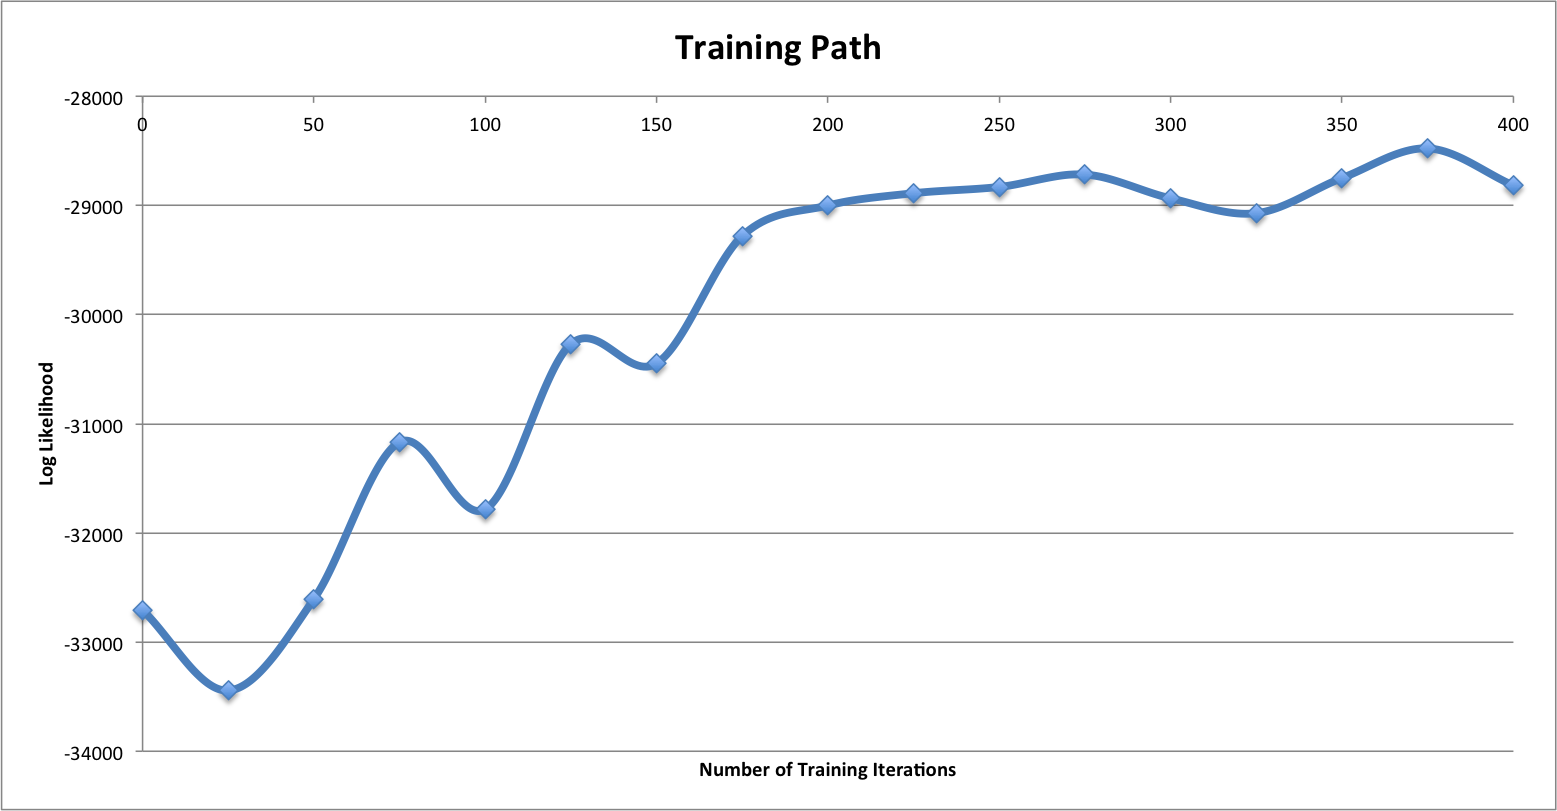
\includegraphics[scale = 0.6]{TrainingPath}
\end{figure}

Moreover, the coefficients all appear to have the correct sign in the model after 400 iterations (noting that positive indicates more likely to vote for Clinton over Trump): 

\begin{table}[H]
\centering
\label{my-label}
\begin{tabular}{|l|l|l|l|l|}
\cline{1-2} \cline{4-5}
\textbf{Coefficient}      & \textbf{Fitted Value} &  & \textbf{Coefficient}         & \textbf{Fitted Value} \\ \cline{1-2} \cline{4-5} 
is Chester resident?      & 0.61                  &  & voted in Democratic primary? & 0.18                  \\ \cline{1-2} \cline{4-5} 
is Adams resident?        & -0.42                 &  & voted in Republican primary? & -0.30                 \\ \cline{1-2} \cline{4-5} 
is Bedford resident?      & -0.78                 &  & is Female?                   & 0.03                  \\ \cline{1-2} \cline{4-5} 
is Allgeheny resident?    & 0.39                  &  & is Male?                     & -0.05                 \\ \cline{1-2} \cline{4-5} 
is registered Democrat?   & 0.30                  &  & Age                          & -0.26                 \\ \cline{1-2} \cline{4-5} 
is registered Republican? & -0.52                 &  &                              &                       \\ \cline{1-2} \cline{4-5} 
\end{tabular}
\end{table}

\section{Next Steps}
(*NITIN CLEAN THIS UP *)
\begin{itemize}
\item Fit models to more data and fit more complex models with more predictors 
\item Evaluate as a prediction task -- fit model to 70\% of the precincts and test on the remaining 30\% of the precincts, using the total number of Trump and Clinton votes in the precinct as the outcome variable. 
\begin{itemize}
\item We're particularly curious if this approach (modeling at the individual level) can yield better predictions than modeling at the precinct level (e.g. by aggregating demographics to the precinct level and then fitting a linear model). 
\item This is where we can make comparisons to more conventional modeling approaches: linear regression, regression trees, and neural nets, all fit at the precinct level 
\end{itemize}
\item Explore other methods for maximizing the log likelihood and see if they perform better in practice. May want to explore numerical gradients and expectation maximization. 
\end{itemize}

\section{CLT Proof}

Define $d_k = \sum_{i = 1}^n d_{k, i}$ to be the number of Democratic votes in precinct $k$, where $d_{k, i}$ is an indicator variable denoting whether person $i$ in precinct $k$ voted Democrat. We know that $d_k$ follows a Poisson Binomial distribution with success probabilities $p_k = (p_{k, 1}, \dots, p_{k, n})$. Define:
\[ s_{k}^2 = \sum_{i = 1}^{n} p_{k, i} (1-p_{k, i}) \] 
We check the Lyapunov CLT condition for the fourth moment: 
\begin{align*}
\lim_{n \to \infty} \frac{1}{s_k^4} \sum_{i = 1}^n E \left( (d_{k, i} - p_{k, i})^4 \right) &= \lim_{n \to \infty} \frac{\sum_{i = 1}^n p_{k, i}(1-p_{k, i}) \left( 3p_{k, i}^2 - 3p_{k, i} + 1 \right)}{\left(\sum_{i = 1}^n p_{k, i} \left( 1- p_{k, i} \right) \right)^2} \stackrel{?} = 0 
\end{align*}

Observe that $3p_{k, i}^2 - 3p_{k, i} + 1 \in (0, 1)$ if $p_{k, i} \in (0, 1)$. Hence, the numerator is strictly less than $\sum_{i = 1}^n p_{k, i} (1 - p_{k, i})$. Hence, if we can guarantee the numerator grows without bound, then this limit is 0 and the Lyapunov CLT applies. We can do so using a simple condition, like enforcing that there is some $\epsilon > 0$ such that $\epsilon < \bar p_i < 1- \epsilon$ for all $i$ (i.e. the mean probability of voting Democrat in a precinct never falls below some low threshold $\epsilon$ or above some high threshold $1-\epsilon$. 

The Lypaunov CLT now tells us that: 
\[ \frac{d_k - \sum_{i = 1}^{n} p_{k, i} }{s_k} \stackrel{d} \longrightarrow N(0, 1) \] 



\end{document}

